\documentclass[]{IEEEtran}
% some very useful LaTeX packages include:
%\usepackage{cite}      
\usepackage{graphicx}   
\usepackage{subfigure} 
\usepackage{url}       
\usepackage{amsmath}    
\usepackage{caption2}
% Your document starts here!
\begin{document}

% Define document title and author
	\title{Weekly Report}
	\author{Adviser: Prof. Yang Wen \\Student: Cheng Wensheng\\ Period: 2018.9.9-9.16
	}
	\markboth{Visual Information Processing Group}{}
	\maketitle

% Write abstract here
\begin{abstract}
	This week I mainly put my effort on improving deep learning methods accuracy of building extraction.
\end{abstract}

% Each section begins with a \section{title} command
\section{Sar contest}
	% \PARstart{}{} creates a tall first letter for this first paragraph
	\PARstart{T}{his} week is the last week of the competition, and we have 2 chances left to upload our software.
	\begin{itemize}
		\item Last week we used data augmentation to augment the small dataset. Specifically, we flipped images horizontally and vertically, besides, we rotated images every $90^{\circ}$. The result had increased by 1.5\%. 
		\item So we tried to rotate images every $30^{\circ}$. With this dataset, we got about 1.5\% increment on validation set. We handed this version of software as the final one.
		\item The final result showed the F1 score of 61.8\%, which ranked 4th. From the result of ship detection, we found that committee had changed the test set since the history version of ship detection showed a different score. This is not so standard. 
		\item After the competition, we have experienced the whole procedure of algorithm competition. We have tried many tricks we only met in papers but haven't tested by ourselves. We are more familiar with the practical situation and corresponding solutions, which are necessary in projects.    
	\end{itemize}
	
	Fig.~\ref{fig:fw} is the final neural network result. Fig.~\ref{fig:rt} is the ground truth image.


% Main Part


\newpage


\begin{figure}
	\vspace{0.5cm}
%	\begin{minipage}[t]{0.5\linewidth}
		\centering
		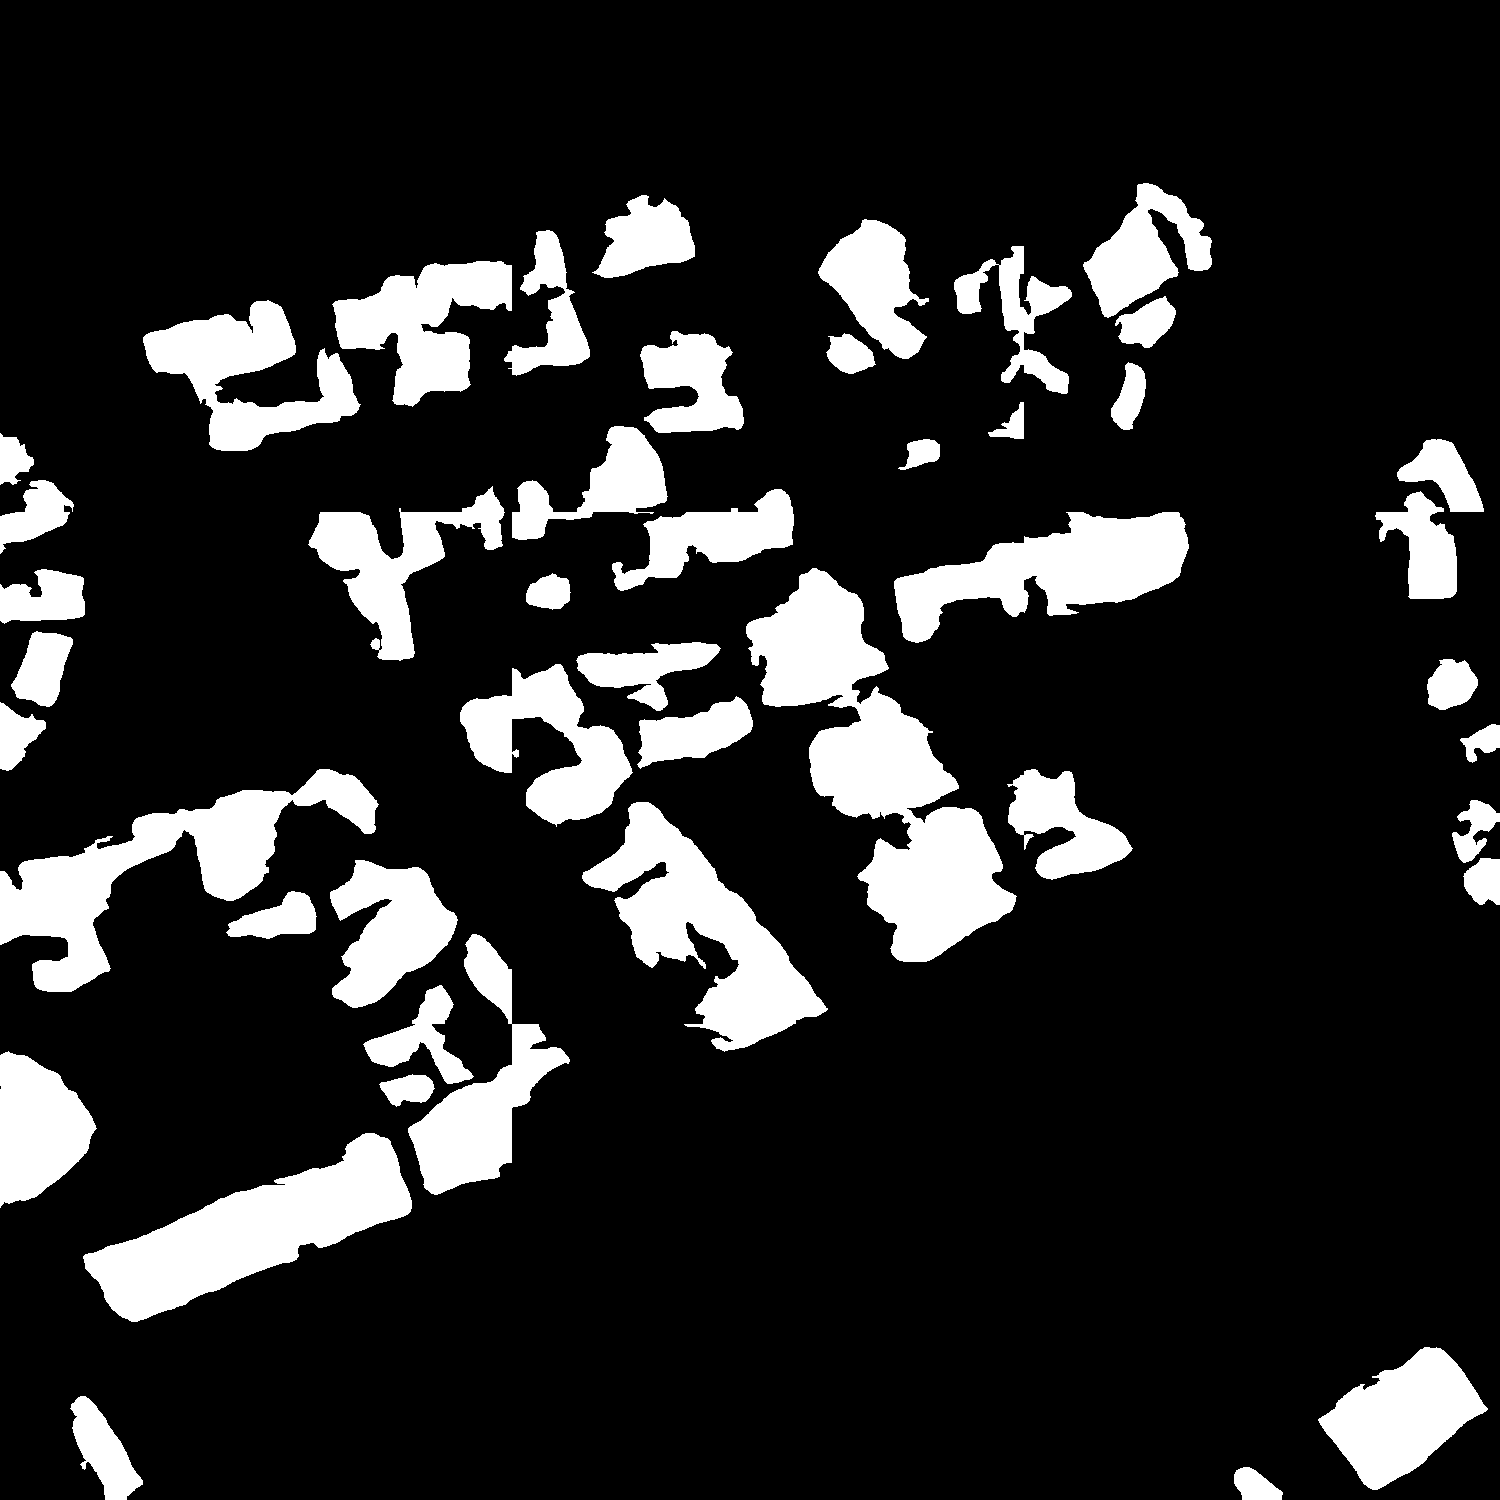
\includegraphics[width=0.7\columnwidth]{fw}
		\caption{Final result}
		\label{fig:fw}
%	\end{minipage}%
%	\begin{minipage}[t]{0.5\linewidth}
	\vspace{0.3cm}
		\centering
		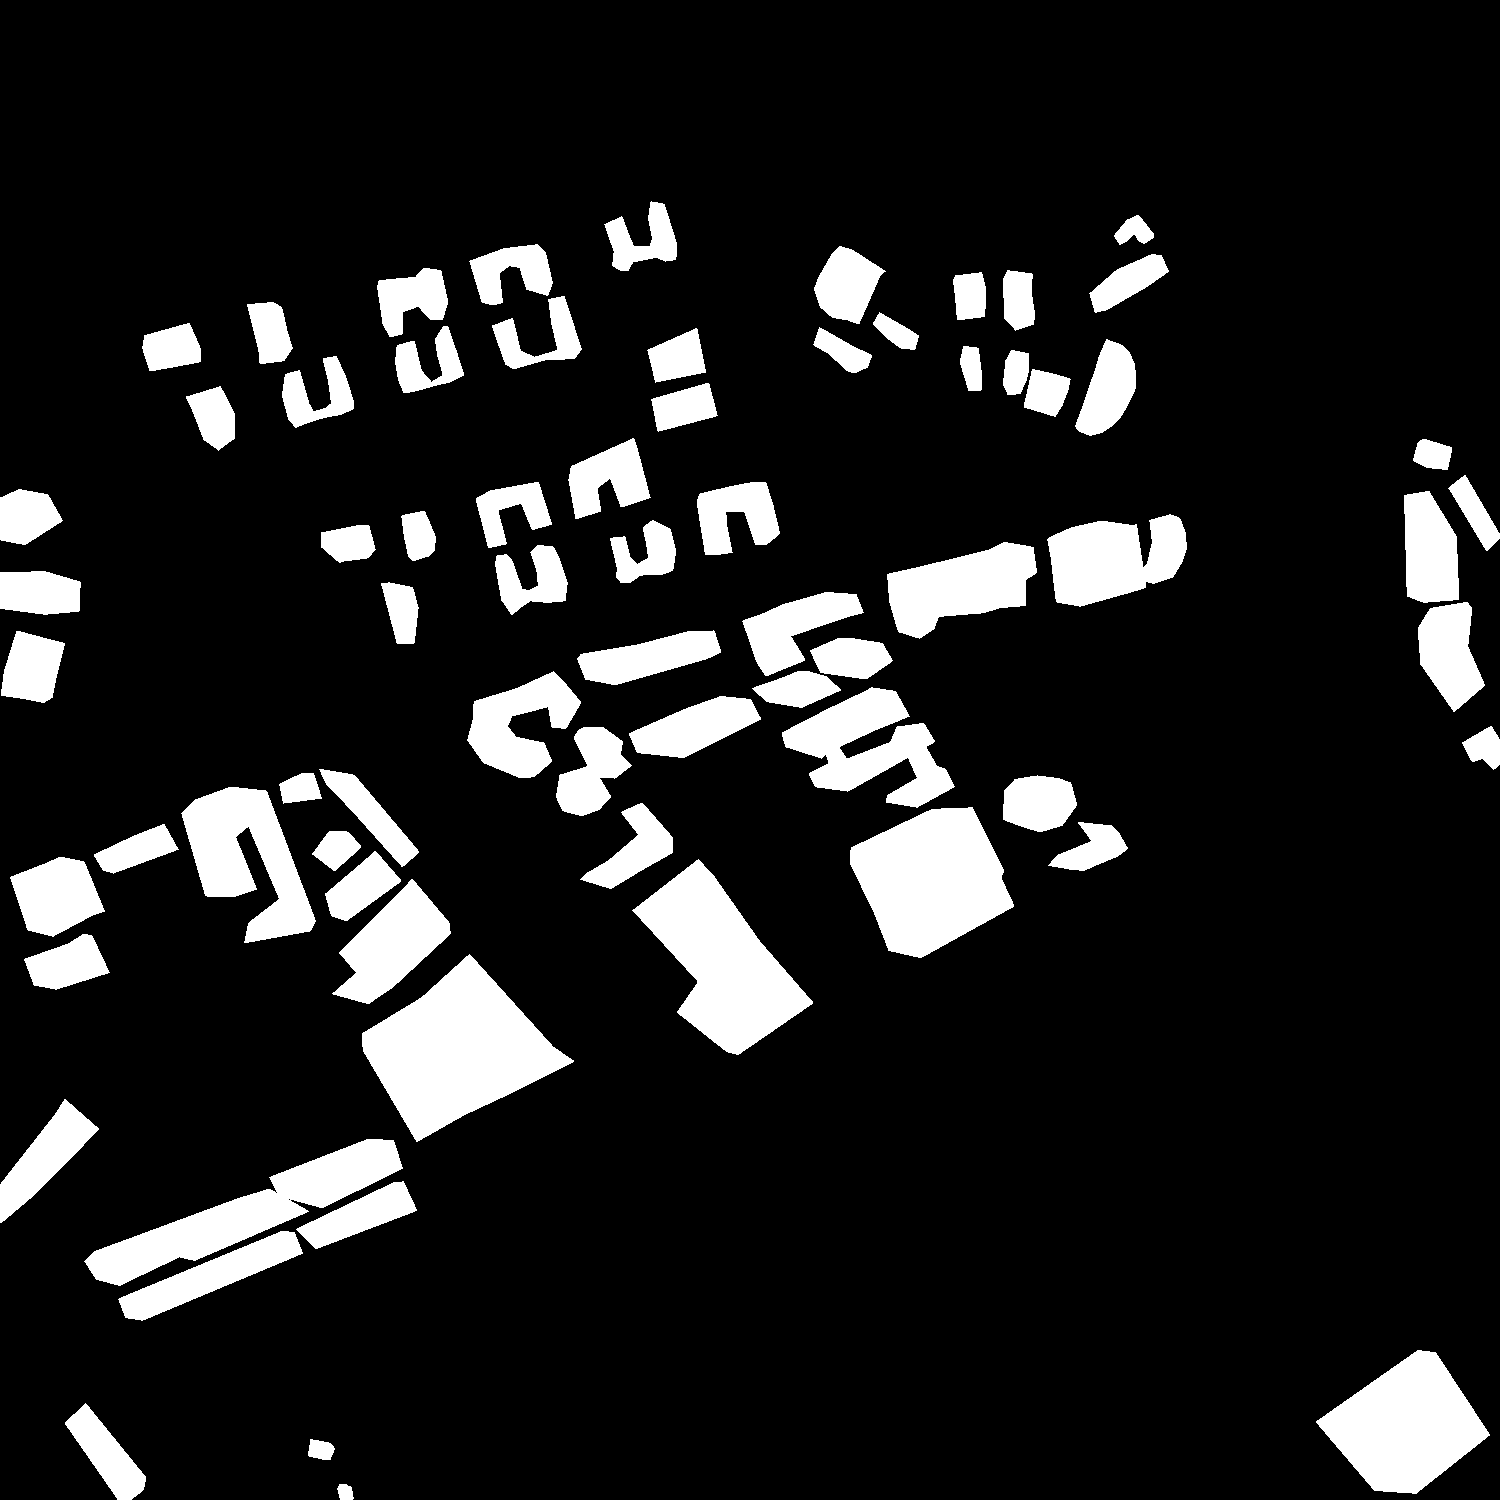
\includegraphics[width=0.7\columnwidth]{rt}
		\caption{Ground Truth}
		\label{fig:rt}
%	\end{minipage}
\end{figure}


%\begin{figure}[!hbt]
%%		 Center the figure.
%		\vspace{0.7cm}
%%		\hspace{50cm}
%		\begin{center}
%			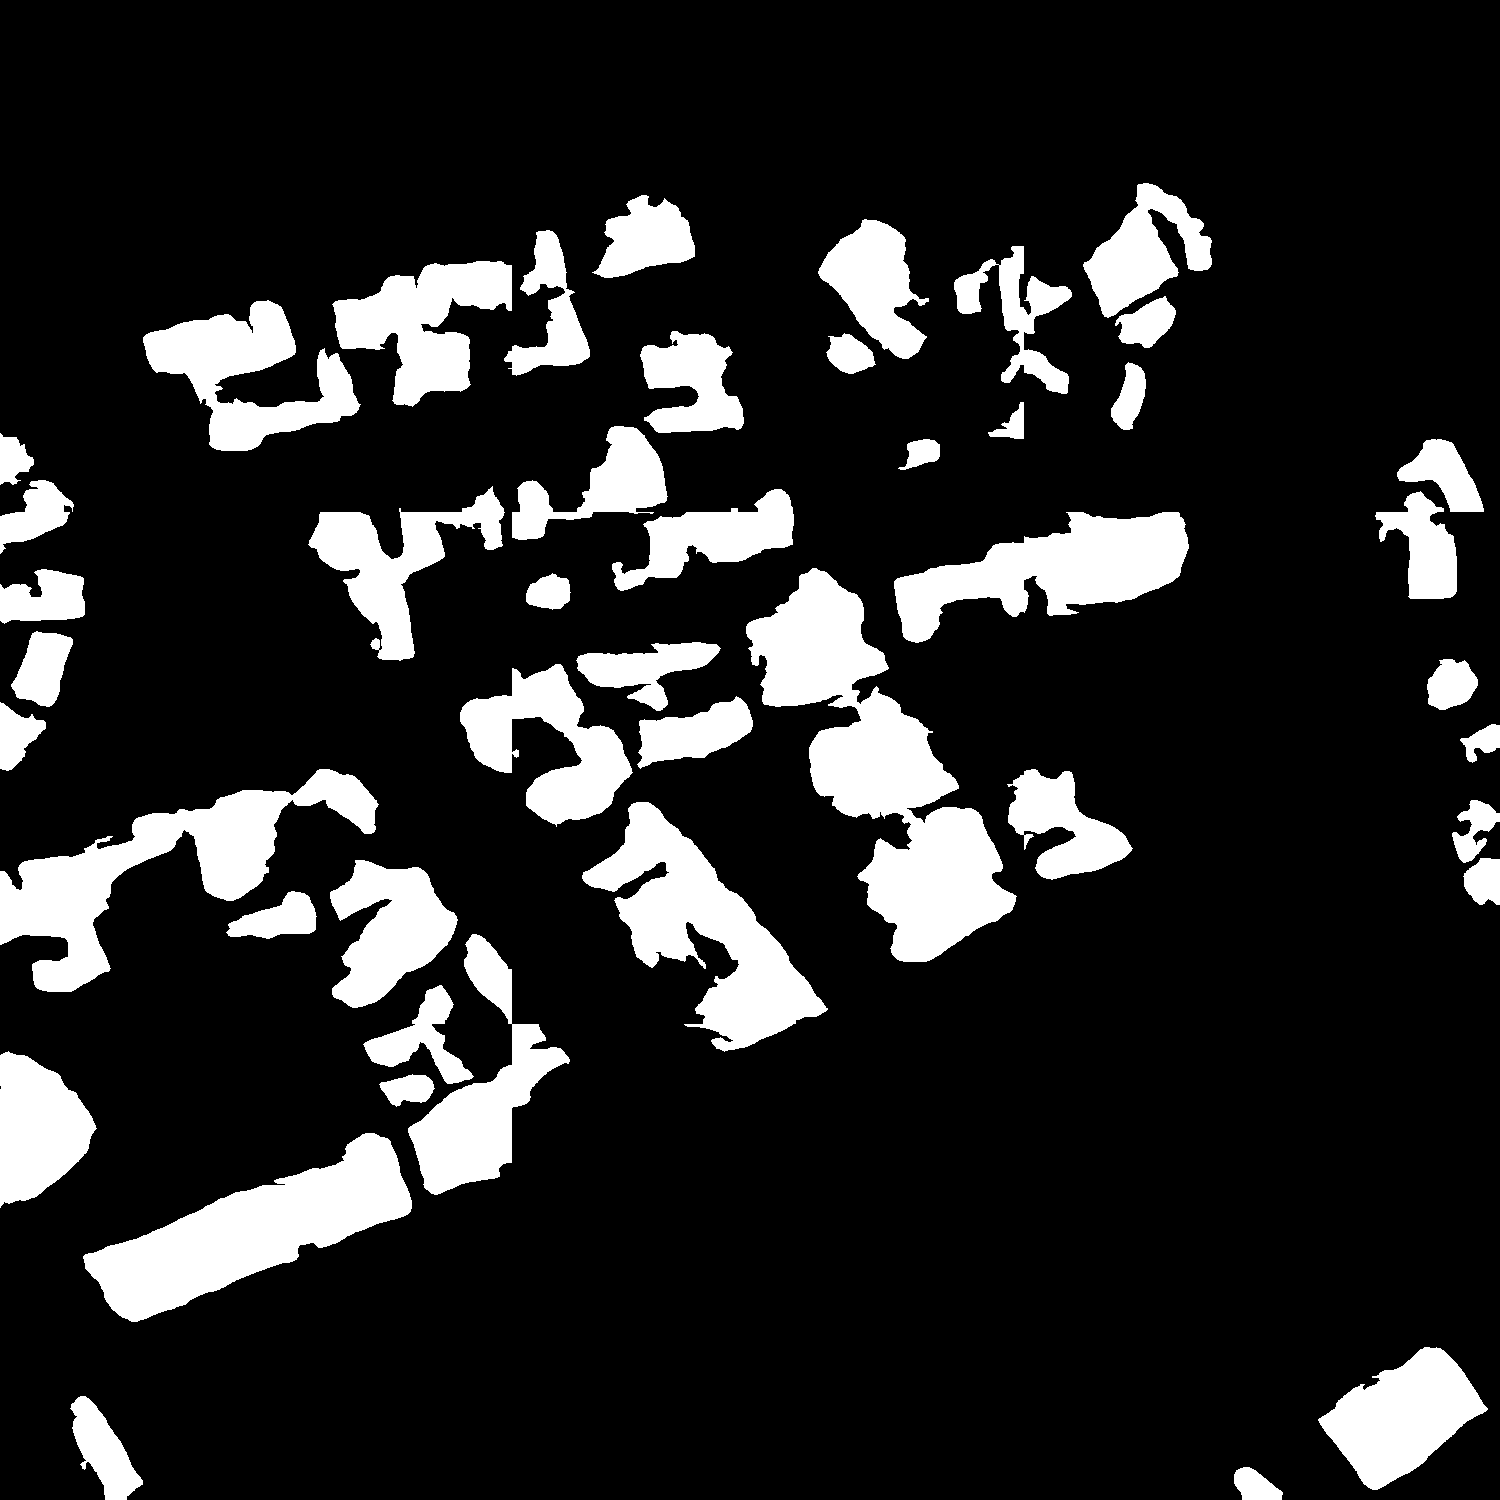
\includegraphics[width=0.2\columnwidth]{fw}
%				%		 Create a subtitle for the figure.
%			\caption{CNN methods result}
%			\label{fig:fw}
%		    \vspace{0.2cm}
%			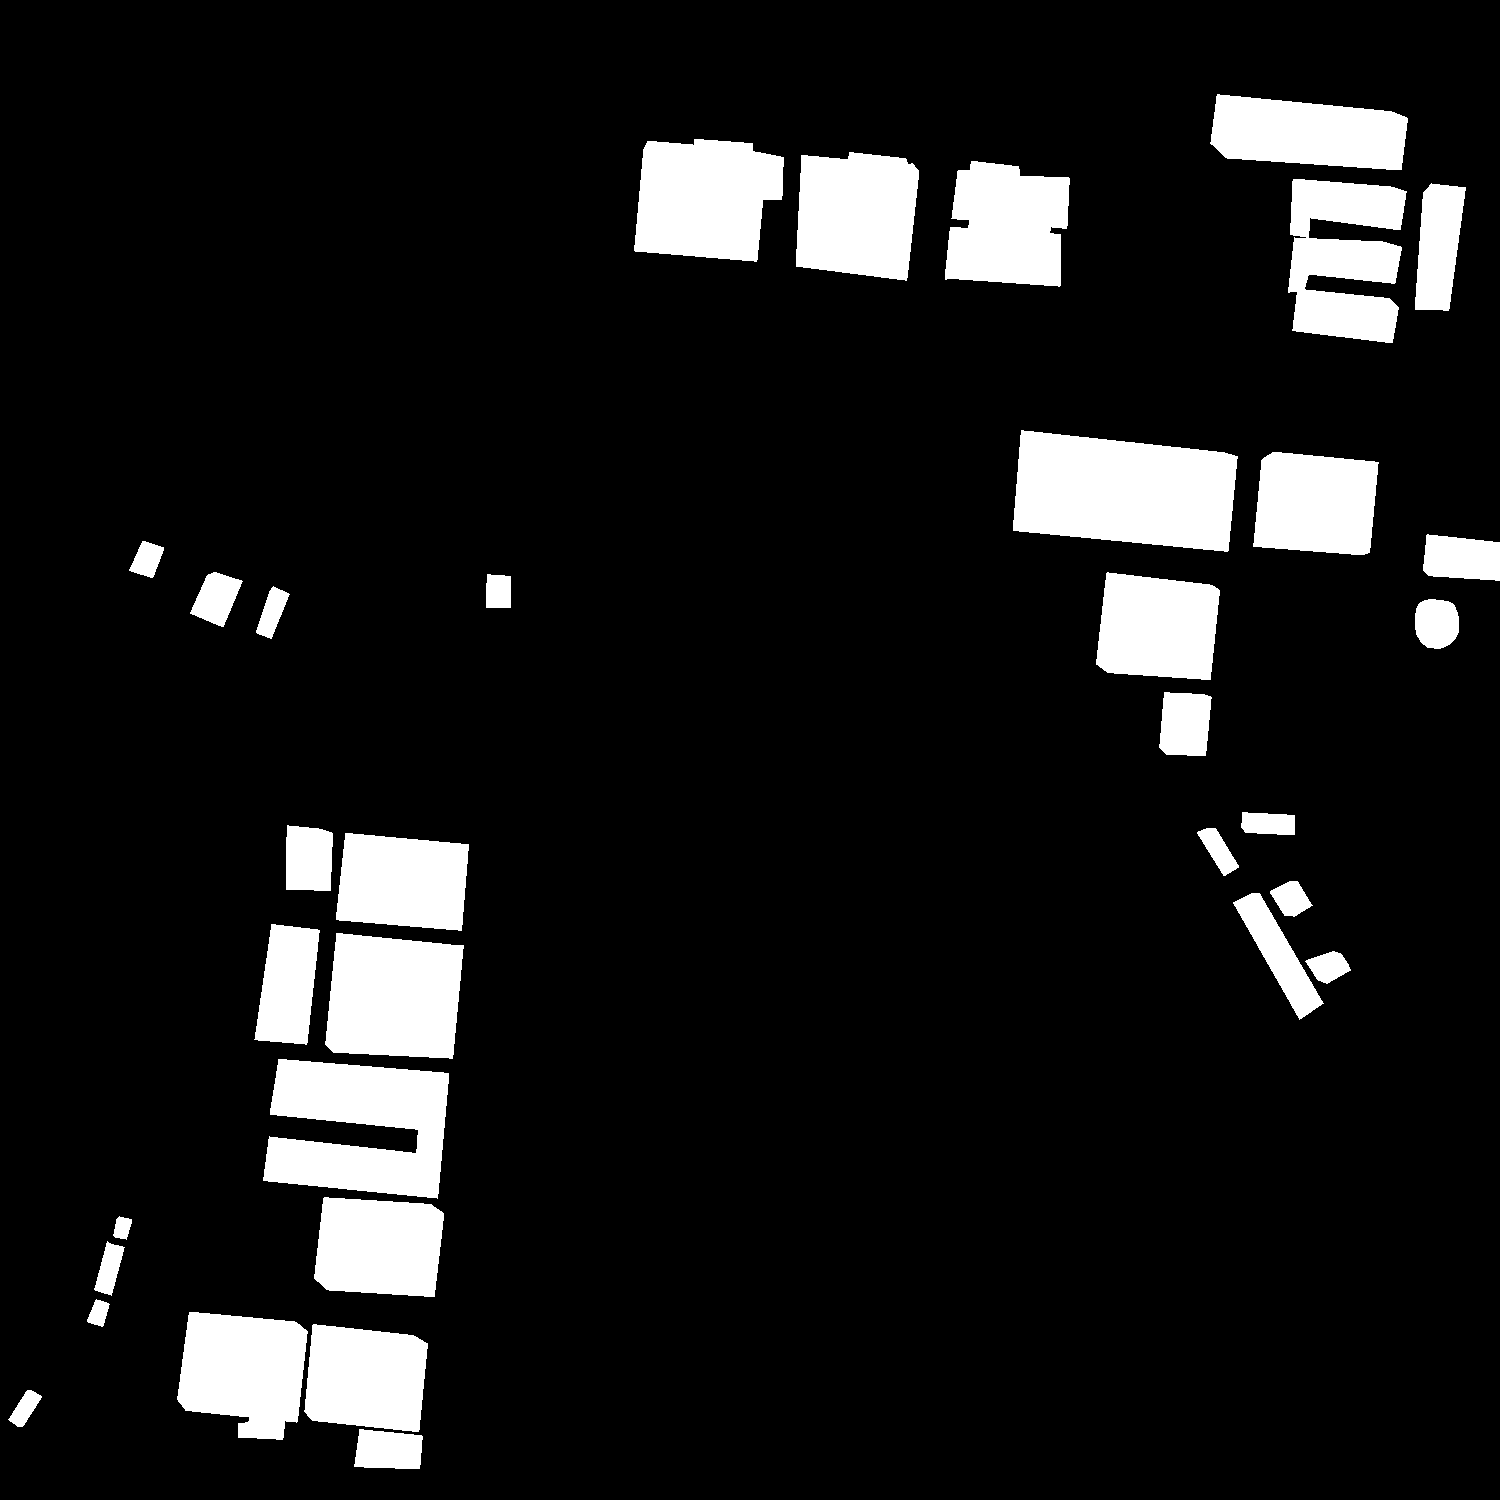
\includegraphics[width=0.2\columnwidth]{rs}
%				%Create a subtitle for the figure.
%			\caption{Ground truth}
%			\label{fig:rt}
%		\end{center}
%	\end{figure}



% Your document ends here!
\end{document}